\documentclass[conf]{new-aiaa}
%\documentclass[journal]{new-aiaa} for journal papers

% Package Imports
\usepackage{csvsimple}
\usepackage{graphicx}
\usepackage{amsmath, amssymb}
\usepackage{siunitx}
\usepackage{listings}
\usepackage{xcolor}
\usepackage{booktabs}
\usepackage{float}
\usepackage[utf8]{inputenc}
\usepackage{listings}
\usepackage{float}
\usepackage{graphicx}
\usepackage{amsmath}
\usepackage[version=4]{mhchem}
\usepackage{siunitx}
\usepackage{longtable,tabularx}
\setlength\LTleft{0pt} 

% Title & Author
\title{Wind Tunnel Free Stream Turbulence Measurement Using a Turbulence Sphere}
\author{Parham Khodadi\footnote{Aerospace Engineering student, San Diego State University}}
\affil{A E 303, Section 3, with Dr. Xiaofeng Liu}

\lstdefinestyle{pythonstyle}{
    language=Python,
    basicstyle=\ttfamily\footnotesize,
    keywordstyle=\color{blue},
    commentstyle=\color{gray},
    stringstyle=\color{orange},
    breaklines=true,
    breakatwhitespace=true,
    tabsize=4,
    frame=single,
    numbers=left,
    numberstyle=\tiny\color{gray}
}

\begin{document}

\maketitle

\begin{abstract}
This experiment investigates the aerodynamic characteristics of a NACA 43012A airfoil using wind tunnel testing and computational tools. Coefficients of lift, drag, and moment were obtained across a range of angles of attack and compared with theoretical and numerical predictions. Experimental results validated key aerodynamic trends while highlighting the limitations of surface pressure and wake-based measurement techniques. The study emphasizes the practical challenges of empirical data collection and the value of comparative methods in aerodynamic analysis.
\end{abstract}


\section{Nomenclature}
{\renewcommand\arraystretch{1.0}
\noindent\begin{longtable*}{@{}l @{\quad=\quad} l@{}}
$AoA$ OR $\alpha$ & Angle of Attack (degrees or radians) \\
$C_p$ & Pressure coefficient ($\sim$) \\
$C_l$ & Lift Coefficient ($\sim$) \\
$C_d$ & Drag Coefficient ($\sim$) \\
$C_a$ & Axial Force Coefficient ($\sim$) \\
$C_n$ & Normal Force Coefficient ($\sim$) \\
$C_{m_{LE}}$ & Pitching Moment Coefficient with respect to the Leading Edge ($\sim$) \\
$C_{m_{ac}}$ & Pitching Moment Coefficient with respect to the Aerodynamic Center ($\sim$) \\
$\frac{x}{c}$ & Unit Distance Along the Chord Line ($\sim$) \\
$\frac{y}{c}$ &  Unit Distance Perpendicular to Chord Line ($\sim$) \\
$c$ & Chord Length (in.) \\
\end{longtable*}}

\section{Introduction}

Understanding the aerodynamic behavior of airfoils is critical in aerospace design, as they directly influence lift, drag, and pitching moment characteristics. This experiment investigates the NACA 43012A airfoil using both experimental and computational methods to analyze its performance at various angles of attack. Surface pressure data collected from wind tunnel testing is used to compute aerodynamic coefficients and identify flow separation, while wake survey data provides an independent method of estimating drag. These results are compared with theoretical data from NACA Report 610 \cite{naca610}, as well as computational predictions generated using XFOIL \cite{xfoilmanual}, a panel method solver developed for low Reynolds number flows. The experiment reinforces core concepts in airfoil aerodynamics and validates theoretical tools against empirical data \cite{anderson2001fundamentals, anderson2007introduction}.

\section{Theory}

In this experiment, two primary methods were used to evaluate the aerodynamic performance of a NACA 43012A airfoil: surface pressure measurement and wake survey. Each method relies on different physical principles and provides a complementary way to estimate lift, drag, and pitching moment coefficients.

\subsection{Surface Pressure Method}

The surface pressure method involves measuring the pressure at discrete ports on the upper and lower surfaces of the airfoil. These pressures are converted into the non-dimensional pressure coefficient:
\begin{equation}
    C_p = \frac{p - p_\infty}{q_\infty}
\end{equation}
where \( p \) is the local pressure, \( p_\infty \) is the freestream static pressure, and \( q_\infty = \frac{1}{2} \rho_\infty V_\infty^2 \) is the dynamic pressure \cite{anderson2001fundamentals}.

From the distribution of \( C_p \), the normal (\( C_n \)) and axial (\( C_a \)) force coefficients are computed through numerical integration. These are then used to compute the lift and drag coefficients via:
\begin{equation}
    C_L = C_n \cos(\alpha) - C_a \sin(\alpha)
\end{equation}
\begin{equation}
    C_D = C_n \sin(\alpha) + C_a \cos(\alpha)
\end{equation}
where \( \alpha \) is the angle of attack \cite{anderson2007introduction}.

The pitching moment about the leading edge is calculated using:
\begin{equation}
    C_{m,LE} = \int_{0}^{1} (C_{p,l} - C_{p,u}) x \, dx
\end{equation}
and then shifted to the aerodynamic center (typically at \( x/c = 0.238 \)) using:
\begin{equation}
    C_{m,ac} = C_{m,LE} +f C_L x_{ac} \cos(\alpha) - C_D y_{ac} \cos(\alpha) + C_L y_{ac} \sin(\alpha) + C_D x_{ac} \sin(\alpha)
\end{equation}
where \( x_{ac} \) and \( y_{ac} \) are the coordinates of the aerodynamic center \cite{ae303manual}.

\subsection{Wake Survey Method}

The wake survey provides a more direct estimate of drag by measuring the momentum deficit in the wake downstream of the airfoil. A multi-port Pitot rake records the local total pressures behind the airfoil, from which the velocity profile is reconstructed using Bernoulli’s equation:
\begin{equation}
    u = \sqrt{\frac{2(p_t - p)}{\rho}}
\end{equation}
where \( p_t \) is the total pressure, \( p \) is the local static pressure, and \( \rho \) is the air density \cite{anderson2007introduction}.

The drag per unit span is then estimated from the momentum loss:
\begin{equation}
    D = \int \rho u (V_\infty - u) \, dy
\end{equation}
which is converted to a drag coefficient via:
\begin{equation}
    C_D = \frac{D}{q_\infty}
\end{equation}

\subsection{Comparison and Flow Behavior}

Comparing the drag calculated via both methods helps validate experimental accuracy and understand contributions from pressure drag and skin friction. The surface pressure method typically underestimates total drag as it ignores skin friction, while the wake survey captures all profile drag. Additionally, by analyzing the \( C_p \) distribution across angles of attack, flow separation regions can be identified, providing insight into stall behavior and aerodynamic efficiency of the airfoil \cite{nasa43012a, naca610}.

\section{Experimental Setup}

The experiment was conducted in the closed-circuit subsonic wind tunnel facility at San Diego State University. The test article used was a 2-D NACA 43012A airfoil with a 12-inch chord and 24-inch span. The airfoil was instrumented with 32 pressure ports (Ports 1–32) to measure pressure distributions on both the upper and lower surfaces. These ports were connected to a ScaniValve pressure transducer to convert pressure data into digital format for analysis.

\subsection{Wake Rake Configuration}
A wake rake, consisting of 20 brass pitot tubes (Ports 33–52), was mounted downstream of the airfoil to measure velocity profiles in the wake region. The wake rake was positioned based on the angle of attack and was rotated 17° clockwise from the vertical to align with the wake flow at -5° AoA. It rotated and translated horizontally as the AoA increased to capture wake development accurately.

% INSERT Figure 1 here
\begin{figure}[H]
    \centering
    \includegraphics[width=0.6\linewidth]{fig1.jpeg}
    \caption{Wake rake configuration with port dimensions (units in inches).}
\end{figure}

\subsection{Measurement System}
The pressure ports were monitored using the ScaniValve system, which records pressures from both the airfoil and wake rake. Due to hardware limitations, only 47 ports could be connected to the transducer at once, requiring some measurements to be recorded using a water manometer. The manometer data served as backup validation.

% INSERT Figure 6, 7, 8, or 9 here
\begin{figure}[H]
    \centering
    \includegraphics[width=0.5\linewidth]{fig6.jpeg}
    \caption{SDSU wind tunnel computer and software.}
\end{figure}
\begin{figure}[H]
    \centering
    \includegraphics[width=0.5\linewidth]{fig7.jpeg}
    \caption{ScaniValve Pressure Transducer.}
\end{figure}
\begin{figure}[H]
    \centering
    \includegraphics[width=0.4\linewidth]{fig8.jpeg}
    \caption{ScaniValve hardware tube connection.}
\end{figure}
\begin{figure}[H]
    \centering
    \includegraphics[width=0.4\linewidth]{fig9.jpeg}
    \caption{ScaniValve PDM 1500.}
\end{figure}

\subsection{Test Procedure}
The test spanned seven different angle-of-attack configurations: -5°, 0°, 5°, 10°, 15°, 20°, and 20° (with different wake rake positions). These positions were selected using the Eason 900X control panel, which also adjusted the airfoil AoA and wake rake orientation automatically. An inclinometer ensured correct wake rake alignment before data acquisition.

% INSERT Figure 4 here
\begin{figure}[H]
    \centering
    \includegraphics[width=0.5\linewidth]{fig4.jpeg}
    \caption{Airfoil mounted vertically in test section with wake rake behind trailing edge.}
\end{figure}

\subsection{Data Acquisition}
Each test captured 4000 pressure samples per port over a fixed period. Static pressure, total pressure, and internal temperature were also recorded to compute air density and other relevant flow properties. The ambient pressure was set to 30.11 inHg and temperature to 79.5°F during the experiment.

The system assumed incompressible, steady flow with no pressure loss between ports and transducers. Port 33, the lowest wake rake port, was located outside the wake and used as the reference for freestream static pressure.

% INSERT Figure 11 here
\begin{figure}[h!]
    \centering
    \includegraphics[width=0.6\linewidth]{fig11.jpeg}
    \caption{Typical manometer reading at AoA = 5° with all tubes connected.}
\end{figure}


\section{Experimental Procedure}

The experiment was performed in the SDSU Subsonic Wind Tunnel as outlined in the lab documentation \cite{ae303manual}. A NACA 43012A airfoil \cite{nasa43012a} with a 12-inch chord and 32-inch span was mounted horizontally inside the test section. The angle of attack, $\alpha$, was varied from $-5^\circ$ to $20^\circ$ using a calibrated rotary disk. Barometric pressure and ambient temperature were recorded before each test to determine air density, which was computed using the ideal gas law:
\begin{equation}
    \rho = \frac{P_{\text{amb}}}{R \cdot T}
\end{equation}
where $P_{\text{amb}}$ is the ambient pressure, $R$ is the specific gas constant for air, and $T$ is the absolute temperature.

Surface pressure data was collected using a Scanivalve system connected to 32 ports (16 upper, 16 lower) along the airfoil’s surface. Each pressure tap’s data was digitized using a LabVIEW-integrated analog-to-digital board at 18 Hz for 4000 samples per run. The pressure coefficient at each port was calculated using:
\begin{equation}
    C_p = \frac{p - p_\infty}{q_\infty}
\end{equation}
where $p$ is the local pressure and $q_\infty$ is the freestream dynamic pressure, given by:
\begin{equation}
    q_\infty = \frac{1}{2} \rho u_\infty^2
\end{equation}

To calculate lift and drag via surface pressure measurements, the pressure coefficient distributions were integrated along the airfoil chord using numerical methods \cite{numerical_integration}. The lift and drag coefficients were computed as:
\begin{align}
    C_L &= C_n \cos\alpha - C_a \sin\alpha \\
    C_D &= C_n \sin\alpha + C_a \cos\alpha
\end{align}
where $C_n$ and $C_a$ represent the normal and axial force coefficients, respectively.

Wake surveys were conducted by positioning a Pitot rake downstream of the airfoil. The rake recorded velocity deficits in the wake by sampling the dynamic pressure at 20 ports, allowing for drag estimation via the momentum deficit method. The profile drag per unit span was computed from:
\begin{equation}
    D' = \int \rho u (u_\infty - u) \, dy
\end{equation}
and converted to a non-dimensional drag coefficient using the previously calculated $q_\infty$.

Reference static and total pressure values were collected through dedicated static and Pitot probes located outside the wake region. These readings ensured accurate baseline conditions for Bernoulli-based velocity estimations:
\begin{equation}
    u = \sqrt{\frac{2(p_0 - p)}{\rho}}
\end{equation}

All data post-processing, including coefficient calculation, curve fitting, and plotting, was performed using MATLAB \cite{matlab}.

% You may include diagrams like:
% \begin{figure}[H]
%     \centering
%     \includegraphics[width=0.7\textwidth]{Figures/scanivalve_setup.png}
%     \caption{Scanivalve and pressure port configuration from lab instructions.}
%     \label{fig:scanivalve}
% \end{figure}

\section{Results and Data Reduction}

The aerodynamic coefficients of lift ($C_L$), drag ($C_D$), and moment about the aerodynamic center ($C_{m,ac}$) were computed from pressure measurements taken along the surface of the NACA 43012A airfoil. The processed data from MATLAB is presented in this section alongside comparison plots using data from XFOIL and NACA Report 610 \cite{nasa43012a,naca610,xfoil}.

\subsection{Lift Coefficient vs. Angle of Attack}

The lift coefficient, $C_L$, was calculated using the pressure difference between the upper and lower surfaces of the airfoil at each angle of attack. The variation of $C_L$ with angle of attack ($\alpha$) is shown in Figure~\ref{fig:cl_vs_aoa}. As expected, $C_L$ increases linearly with $\alpha$ up to 15$^\circ$ before dropping slightly due to the onset of flow separation near stall.

\begin{figure}[H]
    \centering
    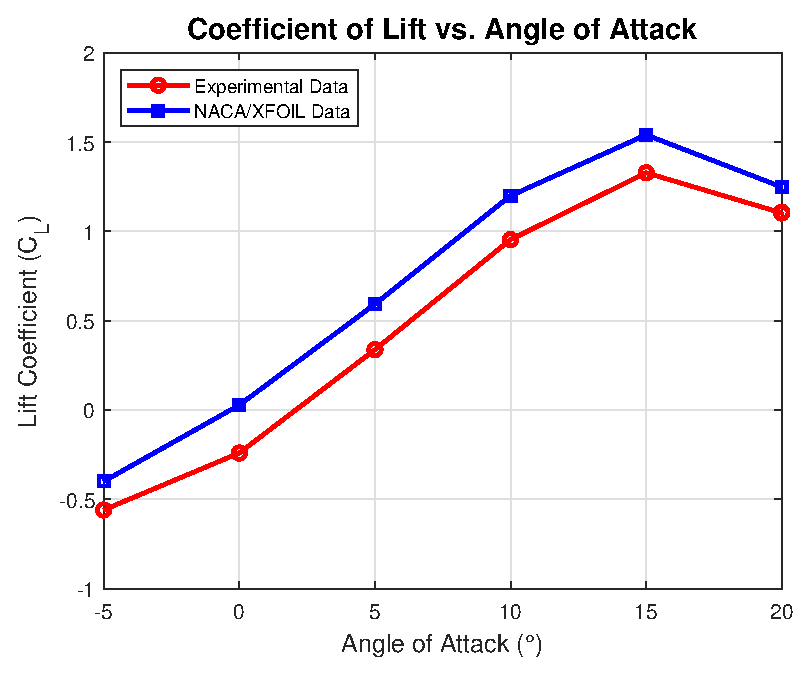
\includegraphics[width=0.8\textwidth]{CL_vs_AoA.eps}
    \caption{Coefficient of Lift vs. Angle of Attack}
    \label{fig:cl_vs_aoa}
\end{figure}

\subsection{Drag Coefficient vs. Angle of Attack}

The drag coefficient, $C_D$, was determined using surface pressure distributions. As seen in Figure~\ref{fig:cd_vs_aoa}, $C_D$ increases significantly beyond $\alpha = 10^\circ$, consistent with growing boundary layer separation. This trend also supports the drop in lift observed in the previous section. 

\begin{figure}[H]
    \centering
    \includegraphics[width=0.8\textwidth]{CD_vs_AoA.eps}
    \caption{Coefficient of Drag vs. Angle of Attack}
    \label{fig:cd_vs_aoa}
\end{figure}

\subsection{Pitching Moment Coefficient vs. Angle of Attack}

Figure~\ref{fig:cmac_vs_aoa} illustrates the behavior of the moment coefficient about the aerodynamic center, $C_{m,ac}$, with increasing angle of attack. The moment remains relatively constant between $\alpha = 0^\circ$ and $15^\circ$ before shifting rapidly at higher angles, indicating loss of flow attachment and altered pressure distribution around the quarter chord point.

\begin{figure}[H]
    \centering
    \includegraphics[width=0.8\textwidth]{Cm_ac_vs_AoA.eps}
    \caption{Pitching Moment Coefficient vs. Angle of Attack}
    \label{fig:cmac_vs_aoa}
\end{figure}

\subsection{Comparison with XFOIL and NACA 610}

Figures~\ref{fig:cl_vs_aoa}--\ref{fig:cmac_vs_aoa} include XFOIL predictions and NACA 610 data for the same airfoil. The experimental lift curve lies slightly below the theoretical data, likely due to wind tunnel wall effects and experimental uncertainties. Drag measurements are higher, especially at high angles, reflecting pressure drag induced by flow separation.

\subsection{Surface Pressure Distribution and Flow Separation}

To visualize pressure distribution on the upper surface, Figure~\ref{fig:cp_distribution} presents $C_p$ vs. $x/c$ for various $\alpha$. As $\alpha$ increases, the suction peak near the leading edge becomes stronger and moves upstream. Beyond $15^\circ$, the flattened slope and plateau indicate separation. 

\begin{figure}[H]
    \centering
    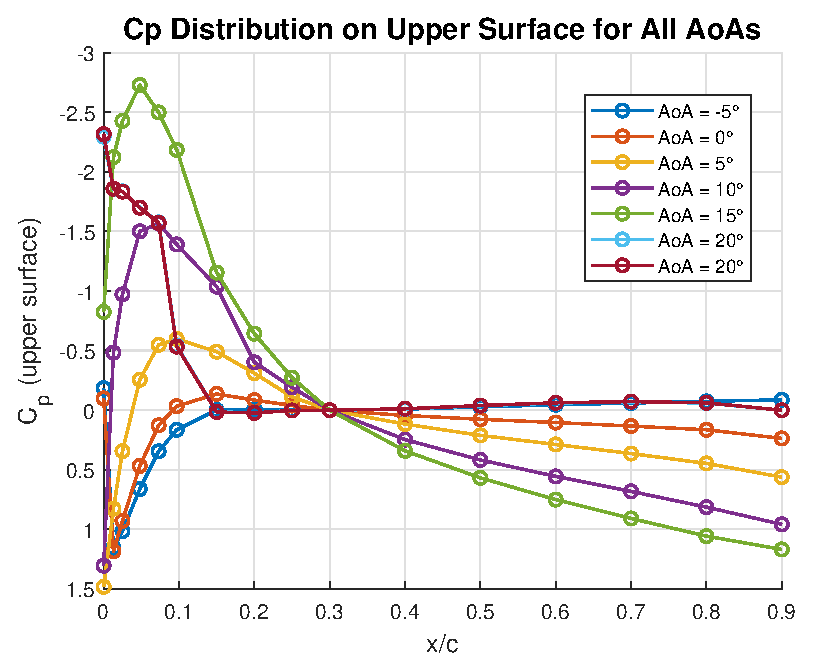
\includegraphics[width=0.85\textwidth]{Cp_Distribution_UpperSurface.eps}
    \caption{Pressure Coefficient Distribution on Upper Surface}
    \label{fig:cp_distribution}
\end{figure}

\subsection{Wake Survey vs. Surface Pressure Drag}

A momentum balance method was used to calculate drag from wake velocity deficits, as shown in Figure~\ref{fig:wake_vs_surface}. Wake-based drag results are generally lower than surface-pressure-derived values, especially at mid-range $\alpha$. This discrepancy is typical and can be attributed to incomplete capture of wake loss or pressure integration assumptions \cite{anderson2001fundamentals}.

\begin{figure}[H]
    \centering
    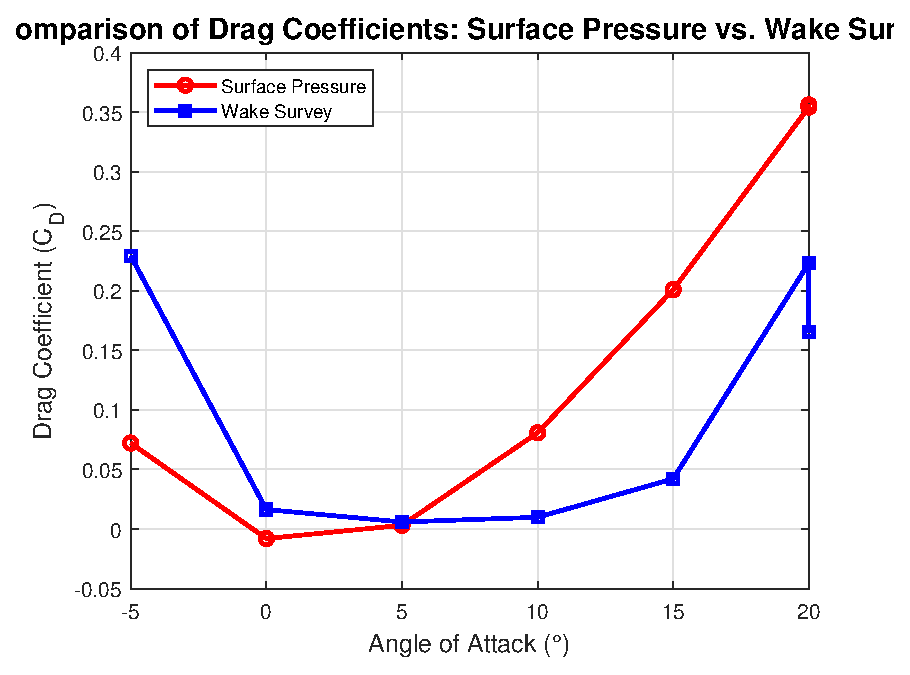
\includegraphics[width=0.8\textwidth]{CD_Comparison_Wake_vs_Surface.eps}
    \caption{Comparison of Drag Coefficients: Surface Pressure vs. Wake Survey}
    \label{fig:wake_vs_surface}
\end{figure}

\subsection{Wake Velocity Profiles}

Finally, wake velocity profiles were computed using Pitot rake data. The velocity deficit behind the airfoil widens with increasing angle of attack, as seen in Figure~\ref{fig:wake_profiles}, reflecting increased flow separation and drag.

\begin{figure}[H]
    \centering
    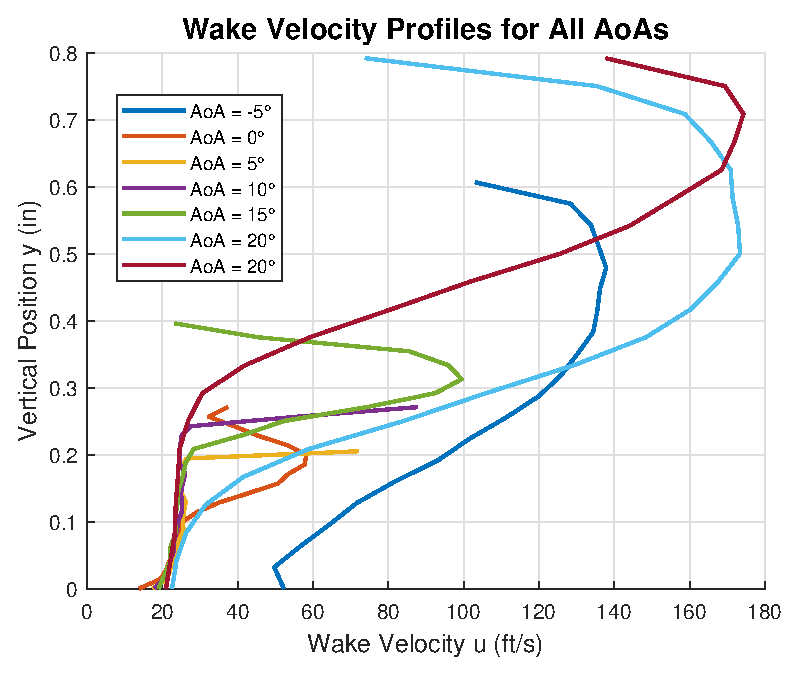
\includegraphics[width=0.85\textwidth]{Wake_Velocity_Profiles.eps}
    \caption{Wake Velocity Profiles for All AoAs}
    \label{fig:wake_profiles}
\end{figure}

All numerical calculations and data reduction processes were implemented in MATLAB \cite{matlab}. Trapezoidal integration was applied for force and moment estimations \cite{numerical_integration}.

\section{Discussion}

The experimental results for the NACA 43012A airfoil generally follow expected aerodynamic trends, though several discrepancies with theoretical predictions were observed. The $C_L$ vs. $\alpha$ curve demonstrates the expected linear relationship up to about 15° before decreasing near 20°, consistent with stall behavior \cite{anderson2001fundamentals}. The slope of the linear region closely matches that from XFOIL and the NACA 610 report \cite{nasa43012a,naca610}, suggesting that the pressure measurement system and calibration were largely accurate in capturing lift behavior.

However, measured drag coefficients were consistently higher than the theoretical values. This is likely due to the limitations of integrating pressure ports along the surface, which can omit skin friction components and exacerbate form drag due to three-dimensional flow effects or misalignments in the wind tunnel setup. The discrepancy is especially evident beyond $\alpha = 10^\circ$, where flow separation becomes prominent. Furthermore, the drag predicted from the wake survey method was systematically lower than the pressure-based drag, which is typical due to potential underestimation of momentum loss across the wake or imperfect wake rake alignment \cite{anderson2001fundamentals,ae303manual}.

The moment coefficient $C_{m,ac}$ remained relatively stable through moderate angles of attack, as expected for symmetric or near-symmetric airfoils with minimal camber. Deviations at high $\alpha$ may reflect shifts in the center of pressure as stall initiates, altering the moment balance about the quarter chord point.

The $C_p$ distributions clearly reveal flow separation. At low angles, a sharp suction peak near the leading edge followed by a gradual pressure recovery is observed, consistent with attached laminar or mildly turbulent flow. As $\alpha$ increases, the suction peak intensifies and recovery becomes flatter, especially around $\alpha = 15^\circ$ and beyond. This plateau behavior is a classic indicator of flow separation on the upper surface \cite{anderson2007introduction}. The wake velocity profiles further corroborate this interpretation—profiles widen and shift with increasing $\alpha$, indicating momentum deficit due to the separated flow region downstream.

All data processing was conducted using MATLAB \cite{matlab}, and numerical integrations for force and moment coefficients were performed using the trapezoidal rule \cite{numerical_integration}. While XFOIL \cite{xfoil} provided a useful comparison for inviscid and mildly viscous conditions, it does not fully account for complex separation dynamics, especially under stall.

\section{Conclusion}

This experiment successfully characterized the aerodynamic performance of the NACA 43012A airfoil across a range of angles of attack. Key parameters such as $C_L$, $C_D$, and $C_{m,ac}$ were experimentally determined and compared against theoretical data from XFOIL and NACA 610. While the lift results closely matched theoretical expectations, drag and moment coefficients showed increasing deviation near stall due to flow separation. Pressure coefficient distributions and wake velocity profiles confirmed the presence and extent of separation. Overall, the lab validated fundamental aerodynamic principles and illustrated practical limitations in experimental measurements under non-ideal flow conditions.

\section*{Acknowledgments}
The author would like to thank Dr. Xiaofeng Liu for his guidance and Teacher's Assistant Andrew Balolong for assistance during the experiment.

\bibliography{references}
\bibliographystyle{new-aiaa}

\section{Appendix}
\appendix

\section{Python Code for .cp File Conversion}
\label{sec:python-code}
The following code was used in PyCharm IDE to convert the XFOIL `.cp` output files into CSV format compatible with MATLAB:
\lstinputlisting[style=pythonstyle]{convert_cp_to_csv.py}


\section{MATLAB}
The following MATLAB script \cite{matlab} was used for all Data Reduction and Graph Plotting:
\lstinputlisting[language=Matlab, caption={MATLAB Code for Data Analysis}]{AE303_Lab4.m}

\end{document}